\chapter{Verloop van het Onderzoek}
\label{onderzoek}

\section{Is het mogelijk om digitaal te gaan?}
\label{onderzoeksvraag1}

Deze sectie gaat na welke methode van geluidsverwerking het best toegepast wordt bij het schrijven van verwerkingsprogramma's. Uit het interview van \textcite{thomashouthave} bleek dat hij het meest intuïtief overweg gaat met subtractive synthesis. In sectie \ref{methode:subtractive} wordt besproken hoe deze methode werkt. \textcite{thomashouthave} meldt in zijn interview dat equalizers en compressors een uitwerking van subtractive synthesis zijn. De andere interviewees vermeldden ook dat zij extensief gebruik maken van equalizers en compressors. Het artikel van \textcite{filtervseq} biedt hier meer inzicht op.

\subsection{Geluidsfilters}

Filters maken prominent deel uit van de subtractive methode zoals in sectie \ref{methode:subtractive} beschreven staat. \textcite{filtervseq} spreekt over de gelijkenissen en verschillen tussen audio equalization en filtering. Waar equalizers bepaalde delen van het frequentiespectrum van een geluid versterken, knippen filters ze af. Beide kunnen gebaseerd worden op een Fast Fourier Transformatie (FFT)\footnote{\textit{fouriereq} leggen in hun onderzoek een toepassing van equalizers uit voor gehoorapparaten. Het idee is om een equalizer in gehoorapparaten te implementeren die bepaalde frequenties verluidt. Die frequenties worden gekozen op basis van het audiogram van de patient. Een audiogram geeft weer vanaf welke amplitude een patient een zekere frequentie kan horen. Zo worden enkel de moeilijk te horen frequenties versterkt. Dit wordt verwezenlijkt door middel van FFT.}. Het enige verschil tussen de twee is de amplitudinale impact. Een equalizer versterkt het geluid rond een zekere frequentie terwijl een filter het verzacht.

Niet alleen biedt FFT meerdere toepassingen in subtractive synthesis. Het biedt ook een tijdscomplexiteit van $\mathcal{O}(n\log{}n)$ die meer acceptabel is dan die van de Discrete Fourier Transformatie (DFT) van $\mathcal{O}(n^2)$.\autocite{ffttime} Het is niet optimaal, daarom worden er reeds tal van onderzoeken gevoerd om de tijdscomplexiteit te verminderen in software aan de hand van multicore computing. \autocite{robbievincke}

De bespreking van FFT is ter illustratie dat equalizers gebaseerd zijn op subtractive synthesis. Er zijn tal van toepassingen van FFT in geluidsfilters maar in software is het typisch niet de verkozen transformatie. Dit omdat het beter gebruikt wordt voor de spectroscopie van frequenties van continue signalen. De sound synthesis libraries besproken in sectie \ref{sec:libraries} maken hier gebruik van de bilineaire tranformatie \autocite{jsynbiquad} omdat die beter toepasbaar is op de real-time verwerking van discrete signalen\footnote{\textcite{rbj} bespreekt in zijn artikel zijn algoritme voor de bilineaire transformatie.}. \textcite{rbj} toont in zijn artikel hoe verschillende filter types geïmplementeerd kunnen worden aan hand van deze transformatie.

\subsection{Harmonisch rijke golven}

Op eerste zicht lijkt het per definitie onmogelijk voor een computer om harmonisch rijke golven te genereren. \textcite{fourier} vertellen het verhaal van Joseph Fourier. In de 19\textsuperscript{de} eeuw stelde hij de hypothese dat alle periodieke functies beschreven kunnen worden als een oneindige som van sinusfuncties - vandaar de benoeming \textit{harmonisch rijk}. Twee jaar voor zijn dood, in 1828, werd dit bewezen door Johann Dirichlet, een wiskundige met wie Fourier correspondentie voerde. Het zijn deze periodieke golven waar subtractive synthesis zich op baseert. \autocite{fourier}

\begin{figure}
\centering
\begin{verbatim}
Function<Double, Double> square = (x) -> (x % p) < (p / 2) ? -1.0 : 1.0;
\end{verbatim}
\caption{Java blokgolf generatie functie}
\label{squarefunction}
\end{figure}

Het is computationeel onmogelijk om een oneindige som van sinusfuncties te genereren.  Maar in se is dat ook niet nodig. Evenals analoge synthesizers genereren de libraries uit sectie \ref{sec:libraries} hun harmonisch rijke golven door middel van logica in plaats van goniometrie. Zo kan de generatie van een harmonisch rijke functie vaak ondergebracht worden in één bewerking. Een voorbeeld in Java: functie \ref{squarefunction} genereert een blokgolf met periode \verb+p+ gegeven een abcis \verb+x+.

De resultaten van deze discrete functies zijn slechts een benadering van die van de continue Fourier series. \autocite{fourier} De geluidsresolutie van vandaag is hoog genoeg dat dit voor het menselijk gehoor nauwelijks zou mogen verschillen. \autocite{vagabundos}

\section{In het nuttig om digitaal te gaan?}

De interviewees hebben elk laten weten wat zij dachten van een digitalisatie. Deze sectie bespreekt aan de hand van hun antwoorden of er in de markt vraag naar is. Het aantal interviews is te klein om een populatie te representeren. Desondanks spreken de interviewees uit jaren van vakkundige ervaring. Daarom kunnen hun antwoorden toch als representabel geacht worden.

\subsubsection{Is het mogelijk om digitaal te gaan?}

Een veel voorkomend argument tegen een digitalisatie is de teloorgang van de fysieke user-interface. Voor muzikanten is dit een natuurlijke reactie. Dit reflecteert bij Adam (Woodie Bundo) Vandenhaute, bassist van Vagabundos: \textit{``For me it's stupid to say but I like the pushing of the pedals. I like the authenticity. With an app that all disappears.''} \autocite{vagabundos} Desondanks is de band wel optimistisch over wat de toekomst te bieden heeft. \textit{``You can still put it all into an iPad and have a pedal to control that. That way you can have the feel, but all the effects are processed by computer,''} aldus Saulo Soneghet, gitarist van Vagabundos. \autocite{vagabundos}

Bart Vincent heeft ook een praktische ingesteldheid ten opzichte van de vraag. Hij zegt het volgende: \textit{``de verwantschap met het instrument gaat anders zijn, maar het gaat nogsteeds een instrument zijn waar je mee om kan leren gaan.''} \autocite{bartvincent}

Peter Boone is iets sceptischer over de digitalisering. \textit{``Op het moment dat de digitalisering begon kon het niet digitaler zijn. [...] Omdat, je sneller een goed resultaat [gaat] behalen met digitale apparatuur dan met analoge apparatuur. Maar ondertussen [...] heb ik gemerkt dat digitale mengtafels het eerste is dat ik heel zwak vindt. Vreselijk ontgoochelend van klank.''} \autocite{peterboone} Hij legt de oorzaak van deze tekortkoming bij de standaardisatie van 44.1 kHz geluidsresolutie. Vooraleer een overstap naar digitaal mogelijk is voor hem, moet eerst die standaard verhoogd worden. Hij is ervan gewaar dat er zulke mengtafels bestaan, maar die zijn volgens hem niet voldoende verspreid en te duur. \autocite{peterboone}

Thomas Houthave spreekt in zijn interview over hybride opstellingen. \autocite{thomashouthave} Hij vertelt dat men niet hoeft te zweren bij analoog of digitaal. \textit{``Alles heeft zijn functies en charmes. Sommige mensen zweren bij analoog maar tegenwoordig staat het zo dicht dat alles subjectief is. Ik vind dat de voor- en nadelen van analoog of digitaal niet in de klank zit maar in het tactiele.''} \autocite{thomashouthave} Het is voor Houthave helemaal mogelijk om digitaal te gaan. De artiest gaat gewoon andere keuzes maken volgens hem. \textit{``Het verschil zit hem in de omgang met het instrument. De user experience heeft ook impact op de keuzes die je maakt.''}

Het aantal parameters dat een interviewee op eenzelfde moment moet bedienen is slechts 1. \autocite{vagabundos} Vincent legt ook uit dat hij alle geluidsinstellingen voor een concert tijdens de PA-repetitie en soundcheck instelt. Verder doet speelt hij een observerende rol die af en toe iets bijstelt waar nodig. Een groter voodeel, volgens Boone, is dat digitale tafels alle instellingen kan opslaan om die op latere momenten met een druk op de knop in te laden.

\subsection{Wie heeft baat bij een digitalisering?}

Evenals Boone ziet Vincent veel potentieel in het digitale voor live performance geluidstechnici. Dit omdat een digitale mengtafel instellingen kan opslaan. \textit{``Als je in een vlugge flow zit op radio, zou het zeker ook kunnen,''} zegt Vincent. \autocite{bartvincent}\newline Boone vindt ook dat de overstap naar digitaal afhangt van het genre van de artiest. \textit{``Met elektronische muziek kan ik mij voorstellen dat je geen boodschap hebt aan analoge toestellen.''} \autocite{peterboone} Zelf zou hij er ook baat bij hebben mits goede geluidsresolutie.

Thomas Houthave heeft zelf al veel ervaring met digitale geluidsverwerking. Desondanks ziet hij nog steeds meer potentieel in software. Hij geeft een aantal creatieve voorbeelden. \textit{``Ik denk niet dat AI op een dag leuke muziek gaat maken. Maar ik denk wel dat je als muzikant of producer tools gaat hebben die het laten lijken alsof je met iemand aan het jammen bent. [...] [Ook] in game engines. [...] De kunst van een game sound designer ligt bij hoe hij de engine kan gebruiken om zijn geluid te vormen.''} \autocite{thomashouthave}

Tijdens het interview stelden Saulo Soneghet en Adam (Woodie Bundo) Vandenhautte zelf al implementaties van digitale effectpedalen voor. In hun rol als muzikant is dat hoever de lijn getrokken wordt omdat intrumenten moeilijk gedigitaliseerd kunnen worden. Saulo Soneghet is gediplomeerd geluidstechnieker en heeft jaren ervaring als producer en muzikant. De band becommentarieerde hem op zijn manier van productie waar hij blijft sleutelen aan zijn geluid tot het ``te perfect'' is. Adam Wilson, zanger van de band, vertelt: \textit{``[...] it didn't sound like us. Saulo loves it cause he can hear his work. [...] he's very proud of it.''} Ze geven Peter Boone als voorbeeld: \textit{``Peter is Peter and he likes another kind of sound so he records it in another kind of way.''} Dit illustreert nogmaals hoe genre en smaak een grote factor spelen in de overstap naar digitaal. Soneghet en Houthave hebben in hun manier van productie meer baat bij de digitalie transitie. Hetzelfde kan ook gelden voor zowel Boone als Vincent afhankelijk van welke projecten ze opnemen. Boone bevestigt het in zijn interview: \textit{``Voor bepaalde genres - industriële popmuziek - is [digitaal] goed, maar voor 'echte muziek' is dat flauwe zever. Het klinkt niet goed. Is mijn mening.''}

\subsection{Zou een digitalisering verwelkomd worden?}

Soneghet is zeer rechtuit in zijn antwoord: \textit{``To me they sound good and to me the final product is most important. You do not need to be a purist. Some say there is a clear difference. Is there?! 99.9\% of the population cannot hear the difference. I challenge the .1\% and I assure you they are bullshitting.''} \autocite{vagabundos} Zoals in sectie \ref{onderzoeksvraag1} besproken werd, bestaan er al technologieën die toe zouden staan om live digitaal geluid te bewerken zonder enig hoorbaar verschil met de analoge variant. Soneghet bevestigt dit.

Boone blijft hier sceptisch over: \textit{``men kan daar zeer gefrustreerd over doen maar de tijd gaat vooruit en het is er, whether you like it or not. Ik ben er wel van overtuigd dat je the best of both worlds moet gebruiken. [...] Dus als je de [financiële] mogelijkheid hebt om dingen analoog te doen zou ik zolang mogelijk in het analoge milieu bezig blijven en pas helemaal op het einde naar digitaal overgaan.''} \autocite{peterboone} Houthave gaat akkoord: \textit{``Het ene moet het ander niet uitsluiten. Ik luister wel naar veel muziek op Spotify maar als ik een album echt mooi vind, dan koop ik het ook op vinyl.''} \autocite{thomashouthave}

Boone voegt hier nog aan toe: \textit{``Pas op, dat geldt voor het genre muziek waar ik aan bezig ben. Maar daarom niet noodzakelijk voor alle genres.''} \autocite{peterboone} Hieruit kan afgeleid worden dat, bij profielen zoals Boone en Vincent, de digitalisering niet zo gegeerd is. Boone ziet echter in dat het voor andere producers wel een handige tool kan zijn. Vincent vertelt over de verwelkoming van de digitalisering: \textit{``het wordt wel verwelkomd maar een computer gaat gewoon nooit het werk van een mens kunnen overnemen. De tools, die de mensen helpen bij hun job, die worden wel beter.''} \autocite{bartvincent} Dit toont aan dat er een interesse is voor digitale tools in de muzieksector. Weliswaar voornamelijk voor live muziek of bepaalde genres.

\section{Is het realistisch om digitaal te gaan?}

Voor dit onderzoek zijn er performantiemetingen uitgevoerd op de drie libraries die beschreven staan in sectie \ref{sec:libraries}. In sectie \ref{subsec:vergelijkinglibraries} werd de gelijkenis in architectuur tussen de drie libraries vergeleken. Toch brachten ze verbazingwekkend verschillende testresultaten op. In deze sectie worden de verwerking van de resultaten besproken. 

Om antwoord te kunnen geven op de onderzoeksvraag, zou slechts één van de libraries moeten slagen op deze test. Slagen voor deze test houdt in dat de library bij iedere testcase aanvaardbaar performant draait. Hou er rekening mee dat de tests op een ietwat zwakke testmachine draaiden die besproken is in sectie \ref{subsec:methodologie:testmachine}.

\subsection{Uitwerking van een Testcase}
\label{calctestcase}

In sectie \ref{subsub:testframework} wordt besproken hoe de testresultaten verkregen zijn. Deze zijn terug te vinden in appendix \ref{ch:testresultaten}. Vervolgens werden er twee smoothing methodes op de testresultaten uitgevoerd zoals besproken in sectie \ref{sec:methodologie:verwerking}. In appendix \ref{ch:smoothing} staan de resultaten van beide deze methodes. Hier wordt de verwerking van één testcase besproken: processor verbruik in testcase 4 van JSyn.

\begin{figure}
    		\centering
    		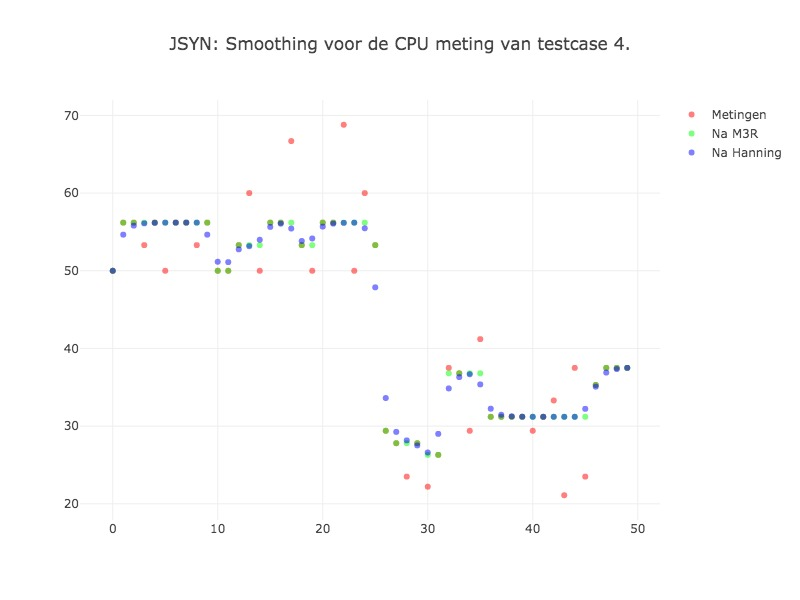
\includegraphics[width=0.75\linewidth]{medians/jsyn_cpu_4}
    		\caption{Smoothing van CPU testresultaten van testcase 4  voor JSyn}
    		\label{jsyn_cpu_4}
\end{figure}

Figuur \ref{jsyn_cpu_4} toont de smoothing van een testcase. De rode punten zijn de originele metingen van de testcase. Als eerste wordt een dubbele \textit{median three smoothing} (M3R) toegepast; besproken in \ref{sec:methodologie:verwerking}. Dit resulteert in de groene set. M3R verwijdert plotse extrema uit het verloop van de meting. Vervolgens is op de resulterende dataset de Hanning vensterfunctie uitgevoerd. Dit leverde de blauwe puntenset op. Hanning maakt dat langere periodes van plotse extrema mooi geëgaliseerd worden.

De mediaan van de dataset die resulteerde uit de Hannign functie werd genomen als resultaat van de meting. In dit voorbeeld is de mediaan \verb+48.93%+. Hieruit kunnen we concluderen dat JSyn doorgaans \verb+48.93%+ van de processorkracht gebruikt op de besproken testmachine.

\begin{table}[]
\centering
\begin{tabular}{l|c|l|l}
\textbf{Library} & \textbf{Case} & \textbf{Mediaan \%CPU} & \textbf{Mediaan \%Mem} \\ \hline
\multirow{6}{*}{\textbf{Beads}} & 1             & 6.23      & 0.70     \\
                           & 2             & 24.12      & 0.80    \\
                          & 3             & 68.80      & 0.80         \\
                          & 4             & 87.50     & 1.10           \\
                          & 5             & 92.59    & 1.50                  \\
                          & 6             & 87.50    & 1.10       \\ \hline
\multirow{6}{*}{\textbf{JASS}}                      & 1             & 93.80     & 0.90          \\
                                                    & 2             & 93.80   & 1.00                    \\
                                                    & 3             & 100.00        & 1.10    \\
                                                    & 4             & 100.00     & 1.20         \\
                                                    & 5             & 100.00                  & 1.30           \\
                                                    & 6             & 100.00      & 1.90           \\ \hline
\multirow{6}{*}{\textbf{JSyn}}                      & 1             & 11.42    & 2.10           \\
                                                    & 2             & 19.05   & 2.30   \\
                                                    & 3             & 33.30     & 2.30         \\
                                                    & 4             & 48.93    & 2.30          \\
                                                    & 5             & 68.81    & 2.30         \\
                                                    & 6             & 56.20    & 2.29       \\ \hline
\end{tabular}
\caption{Medianen van de verwerkte testresultaten per library per testcase.}
\label{medians}
\end{table}

Alle berekende medianen staan in tabel \ref{medians}. Opvallend is dat JASS al snel aan 100\% processor vermogen zit. Waarom wordt duidelijk na het lezen van de broncode. Voor het opstellen van de testcases van JASS is de \verb+Sine+-klasse gebruikt want het is de enige oscillator aanwezig in de library. \textcite{jasscode} vermeldt in de broncode van de klasse dat dit een \textit{``highly inefficient implementation''} is.

\subsection{Trend van de Metingen}

\begin{figure}
    		\centering
    		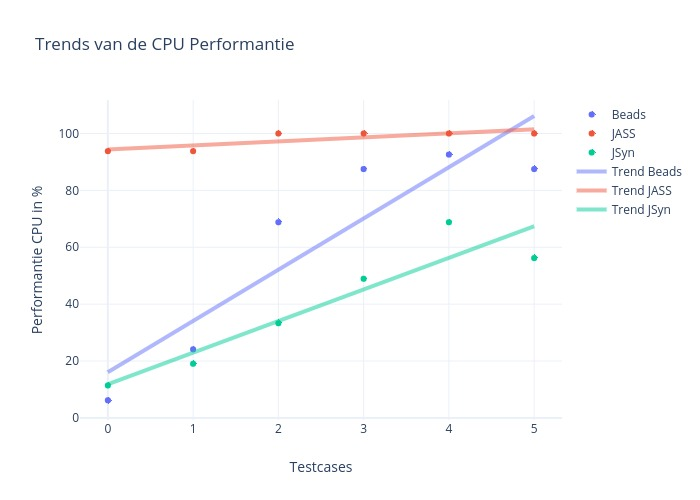
\includegraphics[width=0.75\linewidth]{medians/trendcpu}
    		\caption{Trending van het CPU-verbruik.}
    		\label{trendcpu}
\end{figure}

\begin{figure}
    		\centering
    		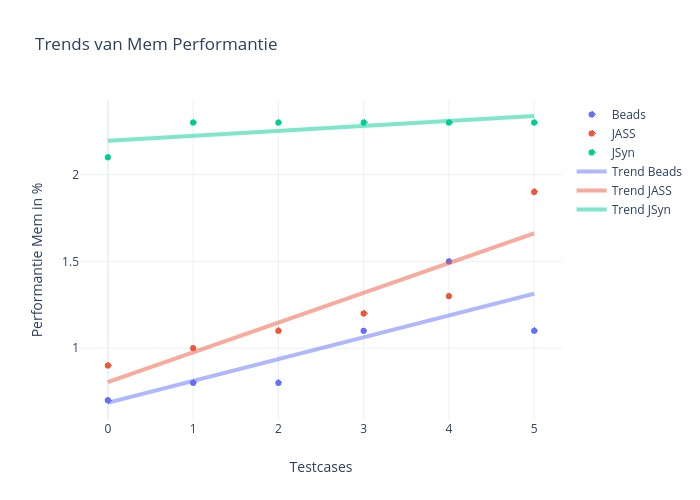
\includegraphics[width=0.75\linewidth]{medians/trendmem}
    		\caption{Trending van het geheugenverbruik.}
    		\label{trendmem}
\end{figure}

De berekende medianen en hun trendlijnen zijn voor zowel de CPU- als geheugenmetingen respectievelijk weergegeven in tabellen \ref{trendcpu} en \ref{trendmem}. Merk op bij tabel \ref{trendmem} dat de metingen niet hoger komen dat 2.3\%. Hoewel JSyn hier wel het hoogste geheugenverbruik heeft, is de stijgende trend van alle libraries toch aanvaardbaar op vlak van geheugen. Geen van deze libraries zullen een tekort aan geheugen veroorzaken in een systeem - zelfs in testcases die meerderemaals de omvang van testcase 6 hebben.

Voor de CPU-metingen is de trendlijn van JASS het eerste dat opvalt. Aan het eind van sectie \ref{calctestcase} werd al verteld waarom. De library voldoet al niet meer aan de eisen voor een hypothetisch eindproduct. Daarom wordt deze meting verder niet in rekening gehouden.

De trendlijn van JSyn is de enige die voor alle testcases onder de lijn van 100\% CPU-verbruik blijft. Een maximum verbruik van 68.81\% is een aanvaardbaar verbruik om geen storingen te geven in live concerten. Daarbij mag vermeld worden dat Beads ook slaagt op de helft van de cases.

